\chapter{Stationary properties} 


\section{Boundary conditions}

To obtain the spectrum of the system it's necessary to find the boundary conditions. As the barrier chemical potential  is the biggest energy parameter of the problem, the wave-functions there are defined by the Hamiltonian:
\begin{gather}
\label{barrier_Hamiltonian}
	H(y)
	=
	\br{
		\frac{p^2}{2m}
		+\mu_b
	}\tau_z,  ~~~~~~~~~-\frac{L}{2}<y<\frac{L}{2}
\end{gather} 

All the majorana physics lives at the energies of the order of $ g $, so that are the energies one should consider in the problem. Because of that the momenta inside the barrier is $ p_b\approx\pm i \sqrt{2m\mu_b} $. One can solve the problem given by (\ref{barrier_Hamiltonian}) and match the values of the wavefunction and it's derivatives on the left and on the right of the barrier to obtain:
\begin{gather}
	\begin{cases}
	\psi_L + b\partial_y\psi_L=t(\psi_R + b\partial_y\psi_R) \\
	\psi_R - b\partial_y\psi_R=t(\psi_L - b\partial_y\psi_L)
	\end{cases}
\end{gather}

here $ \psi_{L,R}=\psi\br{\mp\frac{L}{2}} $, $ b=\frac{1}{\sqrt{2m\mu_b}} $ --- the penetration depth for the particle inside th barrier and $ t = e^{-\frac{L}{b} }$ --- the tunneling constant assumed to be small: $ t\ll 1 $. This condition reads, that the size of the barrier $ L $ should be  much bigger that the penetration depth $ b $.

This condition is invariant under the combined action $ L\leftrightarrow R $, $ y\to-y $. To simplify the further analysis one can reverce th direction in the left wire and put both ands of the wiers from $ y= \frac{L}{2} $ to $ y=0 $. The boundary condition than becomes:
\begin{gather}
\begin{cases}
\psi_L - b\partial_y\psi_L=t(\psi_R + b\partial_y\psi_R) \\
\psi_R - b\partial_y\psi_R=t(\psi_L + b\partial_y\psi_L)
\end{cases}
\end{gather}
This transformation is illustrated on the fig \ref{fig:bctransform}.
\begin{figure}[H]
	\centering
	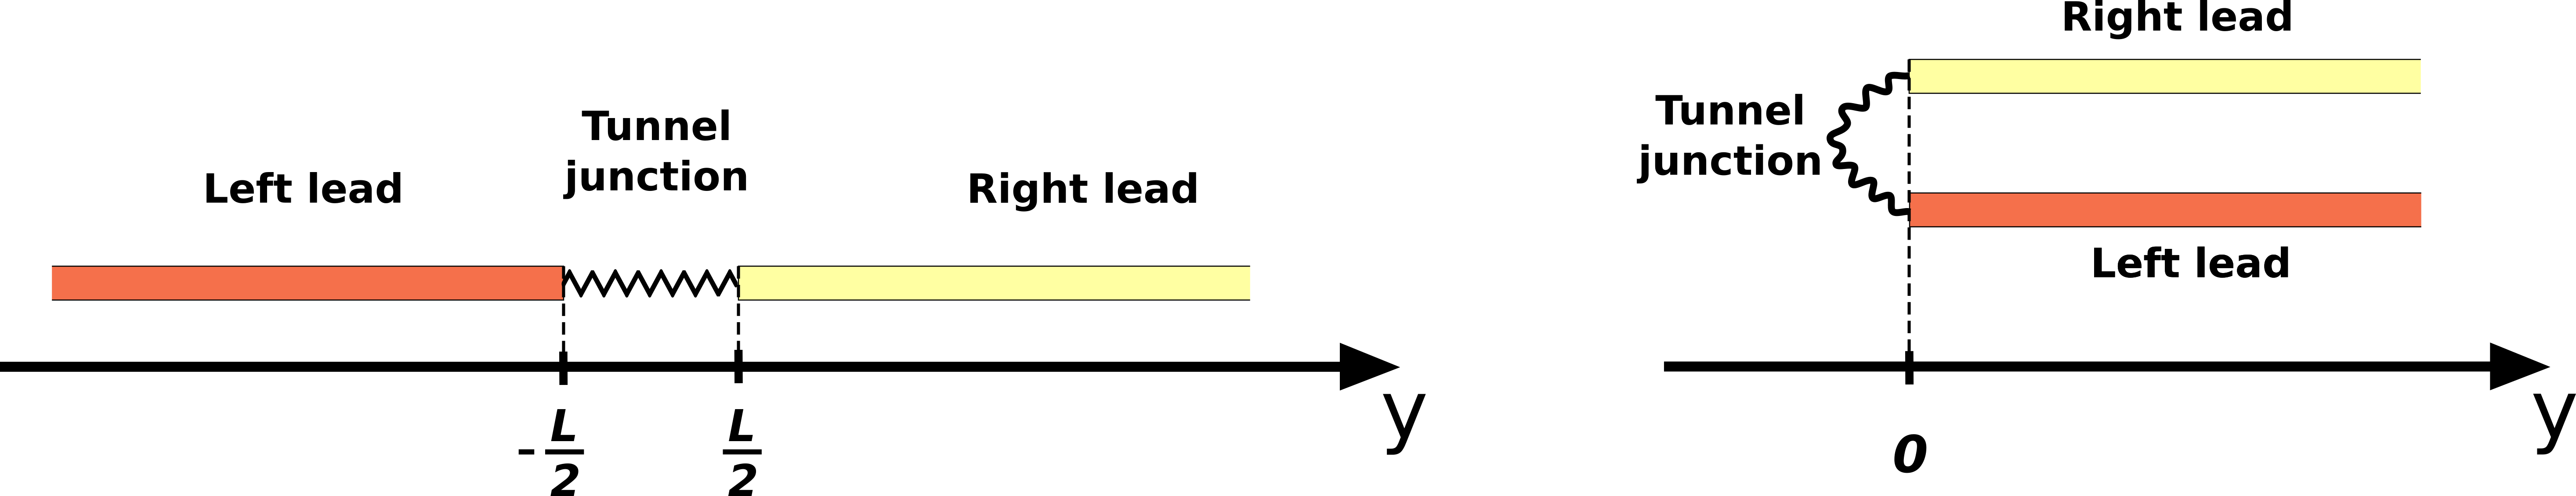
\includegraphics[width=0.9\linewidth]{images/bc_transform}
	\caption{Illustration of switching the deirction of the wire}
	\label{fig:bctransform}
\end{figure}
